\documentclass[border=2pt]{standalone}
\usepackage{tikz}
\usetikzlibrary{quotes,angles}
\usepackage{amsmath}

\begin{document}

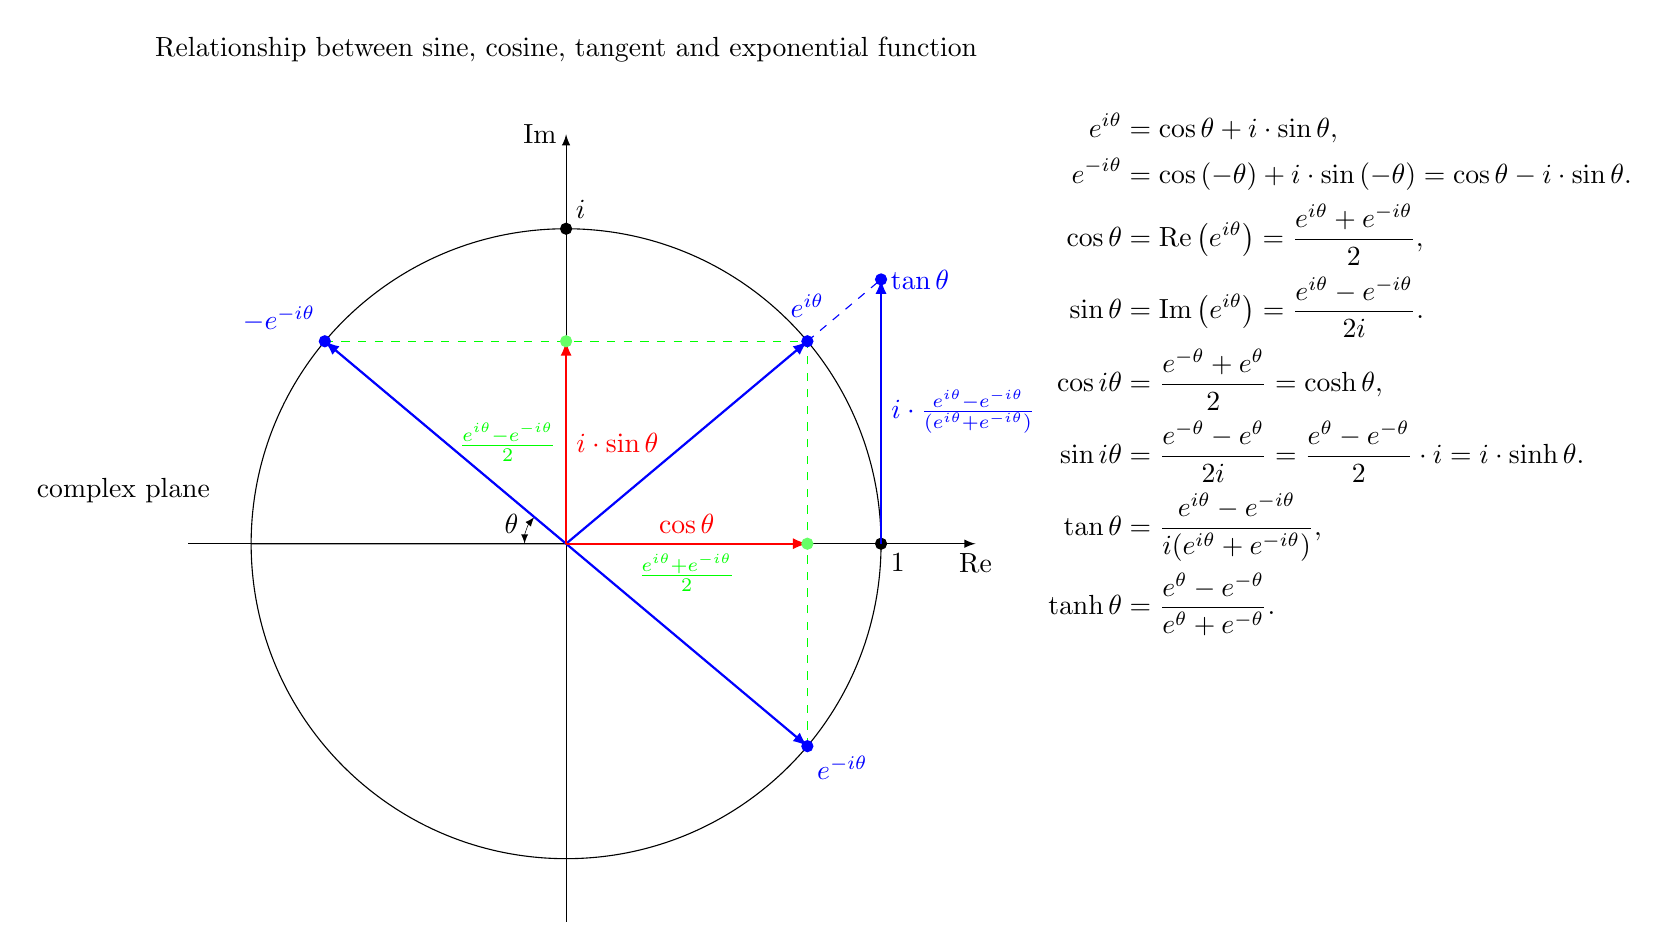
\begin{tikzpicture}[scale=4]

% Draw x and y axis lines
\draw [->,>=latex] (-1.2,0) -- (1.30,0) node [below] {$\mathrm{Re}$};
\draw [->,>=latex] (0,-1.2) -- (0,1.30) node [left] {$\mathrm{Im}$};
\node[above left] at (-1.1, 0.1) {complex plane};
\filldraw[black] (1,0) circle (0.5pt) node[below right] {$1$} ;
\filldraw[black] (0,1) circle (0.5pt) node[above right] {$i$} ;
\node[above] at (0.0,1.50) {Relationship between sine, cosine, tangent and exponential function};

% Draw a circle at the origin of radius 1
\draw (0,0) circle (1);

\pgfmathsetmacro{\angle}{40}


\draw
  (-{cos(\angle)}, {sin(\angle)} ) coordinate (a) 
  -- (0,0) coordinate (b) 
  -- (-1,0) coordinate (c) 
  pic["$\theta$", draw=black, very thin, <->,>=latex, angle eccentricity=1.4, angle radius=15]
  {angle=a--b--c};


\draw [color=blue, thick, ->,>=latex] (0,0) -- ( {cos(\angle)}, {sin(\angle)} ) ;
\draw [color=blue, thick, ->,>=latex] (0,0) -- ( {cos(\angle)},-{sin(\angle)} ) ;
\draw [color=blue, thick, ->,>=latex] (0,0) -- (-{cos(\angle)}, {sin(\angle)} ) ;
\draw [color=blue, thick, ->,>=latex] (1,0) -- node[color=blue, right] {$i\cdot\frac{e^{i\theta}-e^{-i\theta}}{(e^{i\theta}+e^{-i\theta})}$} ( 1, {tan(\angle)} ) ;
\draw [color=blue, thin, dashed] ( {cos(\angle)}, {sin(\angle)} ) -- ( 1, {tan(\angle)} ) ;

\draw [color=green, dashed] ( {cos(\angle)},-{sin(\angle)} ) -- ( {cos(\angle)}, {sin(\angle)} ) ;
\draw [color=green, dashed] (-{cos(\angle)}, {sin(\angle)} ) -- ( {cos(\angle)}, {sin(\angle)} ) ;

\filldraw[blue] ( {cos(\angle)}, {sin(\angle)} ) circle (0.5pt) node[color=blue, above=5pt] {$e^{i\theta}$} ;
\filldraw[blue] (-{cos(\angle)}, {sin(\angle)} ) circle (0.5pt) node[color=blue, above left ] {$-e^{-i\theta}$} ;
\filldraw[blue] ( {cos(\angle)},-{sin(\angle)} ) circle (0.5pt) node[color=blue, below right] {$e^{-i\theta}$} ;
\filldraw[blue] ( 1, {tan(\angle)} ) circle (0.5pt) node[color=blue, right] {$\tan\theta$} ;

\draw [color=white] (0,0) -- node[color=green, below] {$\frac{e^{i\theta}+e^{-i\theta}}{2}$} ( {cos(\angle)}, 0 ) ;
\draw [color=white] (0,0) -- node[color=green, left ] {$\frac{e^{i\theta}-e^{-i\theta}}{2}$} ( 0, {sin(\angle)} ) ;


\draw [color=red, thick, ->,>=latex] (0,0) -- node[above] {$\cos\theta$} ( {cos(\angle)}, 0 ) ;
\draw [color=red, thick, ->,>=latex] (0,0) -- node[right] {$i \cdot \sin\theta$} ( 0, {sin(\angle)} ) ;

\filldraw[green!60] ( {cos(\angle)}, 0 ) circle (0.5pt) ;
\filldraw[green!60] ( 0, {sin(\angle)} ) circle (0.5pt) ;

\node[below right] at (1.50,1.40) {$
\begin{aligned}
e^{i\theta}&=\cos\theta+i\cdot\sin\theta,\\
e^{-i\theta}&=\cos\left(-\theta\right)+i\cdot\sin\left(-\theta\right)=\cos\theta-i\cdot\sin\theta.\\
\cos\theta&=\mathrm{Re}\left(e^{i\theta}\right)=\frac{e^{i\theta}+e^{-i\theta}}{2},\\
\sin\theta&=\mathrm{Im}\left(e^{i\theta}\right)=\frac{e^{i\theta}-e^{-i\theta}}{2i}.\\
\cos i\theta&=\frac{e^{-\theta}+e^{\theta}}{2}=\cosh\theta,\\
\sin i\theta&=\frac{e^{-\theta}-e^{\theta}}{2i}=\frac{e^{\theta}-e^{-\theta}}{2}\cdot i=i\cdot\sinh\theta.\\
\tan\theta&=\frac{e^{i\theta}-e^{-i\theta}}{i(e^{i\theta}+e^{-i\theta})},\\\tanh\theta&=\frac{e^{\theta}-e^{-\theta}}{e^{\theta}+e^{-\theta}}.
\end{aligned}
$};

\end{tikzpicture}

\end{document}

